% (c) Jeremy Jacob
% This file is made available for educational purposes
% It may not be distributed for profit, or without this header.

% Altered by Daniel Brown.

\documentclass[aspectratio=1610]{beamer}
\usepackage[T1]{fontenc}
\usepackage[british]{babel}
\usepackage[sc]{mathpazo}
\usepackage[scaled=0.9]{helvet}
\usepackage{courier,textcomp,amsmath,listings, color}
\newcommand{\code}[1]{\texttt{#1}}
\setbeamertemplate{caption}[numbered]


% THEME SET UP
% University colours
\definecolor{UoYgreen}{cmyk}{0.82,0.00,0.64,0.70} % Pantone 567
\definecolor{UoYblue} {cmyk}{1.00,0.72,0.00,0.32} % Pantone 281
% Departmental colours
\definecolor{UoYCSbrightgreen}{cmyk}{0.46,0.17,1.00,0.01}
\definecolor{UoYCSyellowgreen}{cmyk}{0.16,0.02,0.51,0.00}
\definecolor{UoYCSgrey}       {cmyk}{0.00,0.00,0.00,0.60}
\definecolor{UoYCSblue}       {cmyk}{0.99,0.68,0.28,0.10}

\usetheme[secheader]{Boadilla}
\usecolortheme[named=UoYCSblue]{structure}
\setbeamertemplate{navigation symbols}{} %removes navigation buttons

% CODE HIGHLIGHTING COLOURS SET UP
% Set up for C#, Credit: http://tex.stackexchange.com/questions/124953/syntax-highlighting-in-listings-for-c-that-it-looks-like-in-visual-studio
%\setmonofont{Consolas} %to be used with XeLaTeX or LuaLaTeX
\definecolor{bluekeywords}{rgb}{0,0,1}
\definecolor{greencomments}{rgb}{0,0.5,0}
\definecolor{redstrings}{rgb}{0.64,0.08,0.08}
\definecolor{xmlcomments}{rgb}{0.5,0.5,0.5}
\definecolor{types}{rgb}{0.17,0.57,0.68}

\lstset
{
  language=Ruby,
  captionpos=b,
  %numbers=left,
  %numberstyle=\tiny,
  frame=lines,
  showspaces=false,
  showtabs=false,
  breaklines=true,
  showstringspaces=false,
  breakatwhitespace=true,
  escapeinside={(*@}{@*)},
  commentstyle=\color{greencomments},
  morekeywords={partial, var, value, get, set},
  keywordstyle=\color{bluekeywords},
  stringstyle=\color{redstrings},
  basicstyle=\ttfamily\small,
}

%Presentation information
\title[EpsilonGit]{Advanced Querying and Analysis of Git Repositories}
\author[Daniel Brown]{Daniel Brown\\{\footnotesize Supervised by: Dr. Dimitris Kolovos}}


\institute[UoY, CS]{The University of York, Department of Computer Science}
\date{\today}

\begin{document}
\frame{\titlepage}

\section{Introduction} %Section title on top of each slide
\begin{frame}
	\frametitle{Outline of Presentation}
	\begin{enumerate}
		\item Literature Review \begin{enumerate}
									\item What is Git?
									\item Existing Solutions for Querying and Analysing Git
									\item What Is Model Driven Engineering \& Epsilon?
								\end{enumerate} 
		\item Problem Analysis \& Motivation
		\item Requirements \& Introducing EpsilonGit
		\item Design, Implementation and Challenges
		\item Example Query and Analysis Code
		\item Comparison to Existing Solutions
		\item Evaluation, Interpretation and Conclusion
		\item Q\&A
	\end{enumerate}
\end{frame}

\section{Literature Review}
\begin{frame}
	\frametitle{What is Git?}
	\begin{enumerate}
		\item Distributed Version Control System
		\item Internally an Content Addressable Filesystem comprising of Blobs, Trees, Commits and Tags [S. Chacon and B. Straub, 2014]
		\item Cornerstone of the development process for millions of users managing millions of repositories including on Social Coding platform Github [B. Doll, 2013].
		\item Growing...
	\begin{figure}[H]
		\centering
		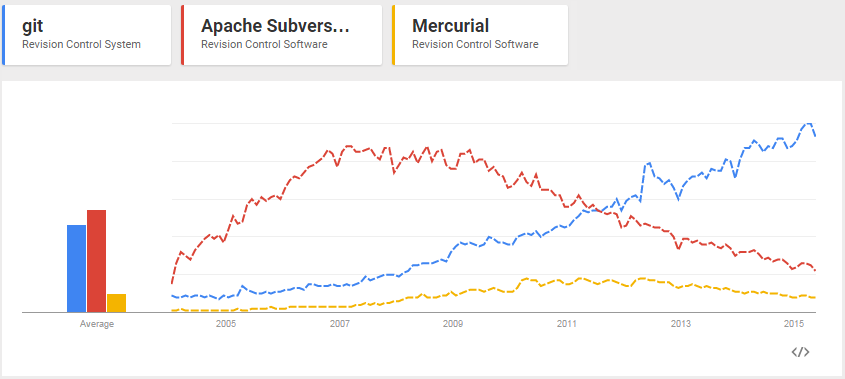
\includegraphics[width=250px]{images/git-google-trends.png}
		\caption{The growth of Git relative to other popular version control systems (Google Trends)}
	\end{figure}
	\end{enumerate}
\end{frame}

\begin{frame}
	\frametitle{Existing Solutions for Querying and Analysing Git}
	\begin{enumerate}
		\item Projects hosted in Github can use Github Graphs
		\item Local solutions include GitInspector and Gitana
		\item Most people just use the built in \code{git log} command
	\end{enumerate}
	\begin{figure}[H]
		\centering
		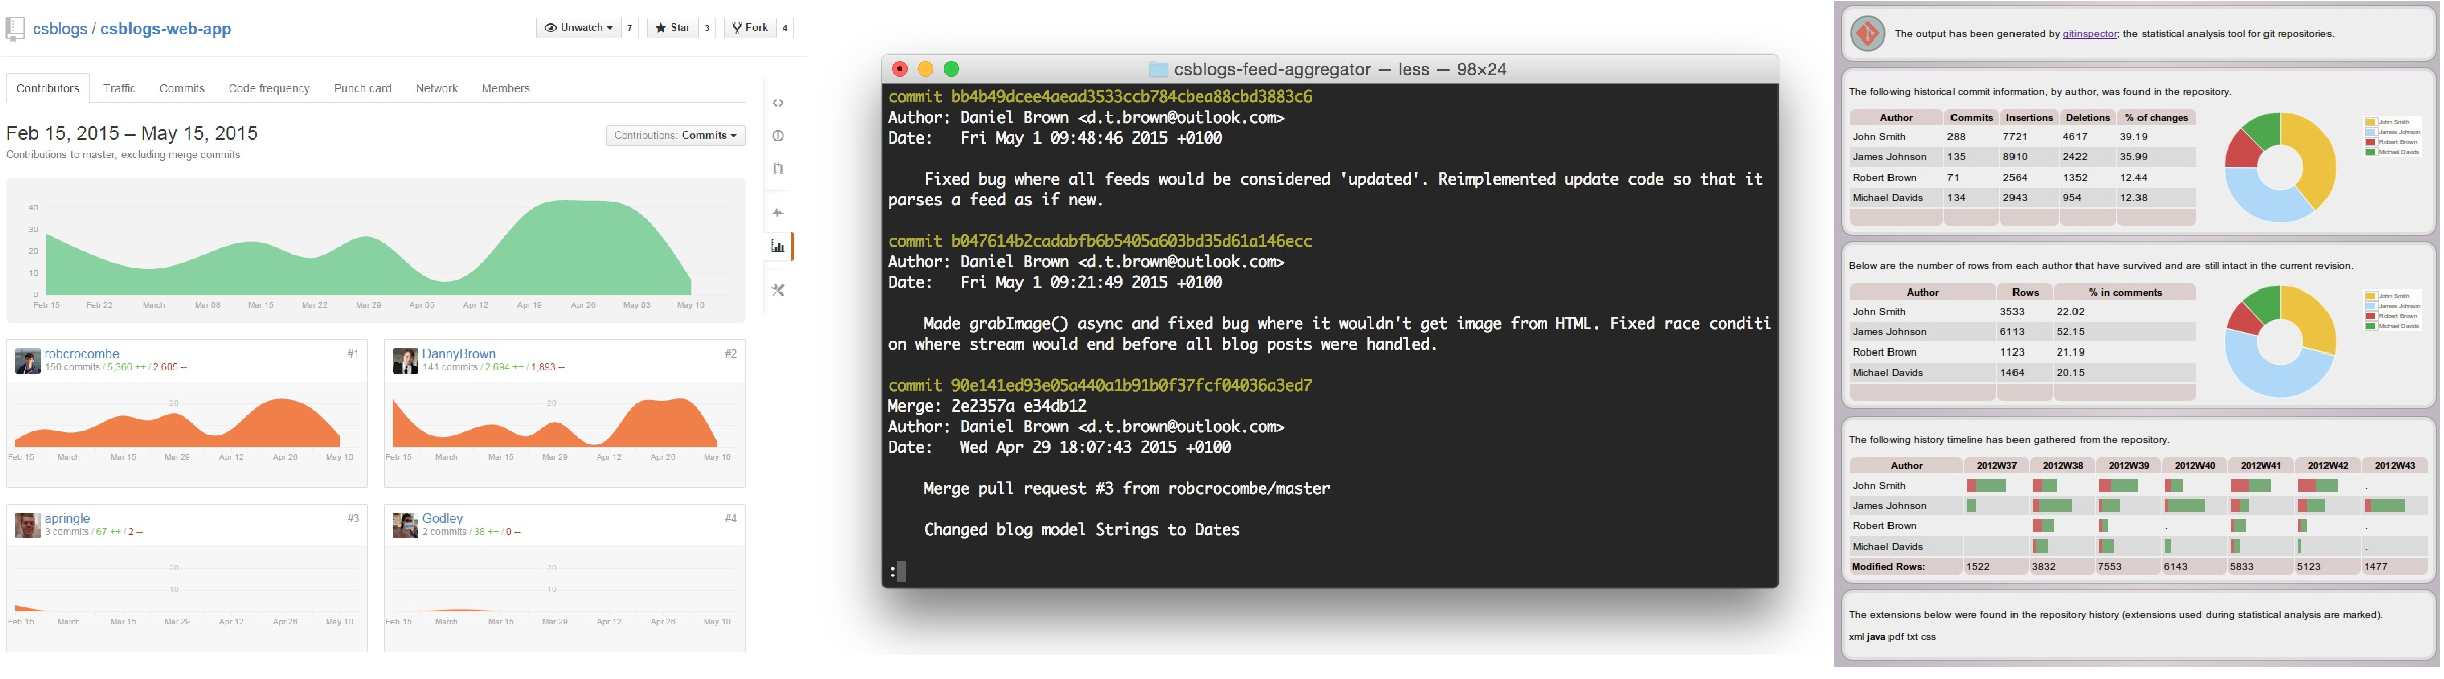
\includegraphics[width=350px]{images/existingsolutions}
		\caption{The output of Github Graphs, the \code{git log} command and GitInspector}
	\end{figure}
\end{frame}

\begin{frame}
	\frametitle{What Is Model Driven Engineering \& Epsilon?}
	\begin{center}
	
\includegraphics[width=140px]{images/epsilon}
	\end{center}
	\begin{enumerate}
		\item Model Driven Engineering is an approach to tackle the complexity of data, and how it is inter- acted with, through the use of high level abstractions called models and a set of Domain- specific modelling languages and Transformation engines and generators [D. C. Schmidt, 2006].
		\item Epsilon is a family of languages and tools for code generation, model-to-model transformation, model validation, comparison, migration and refactoring working on models and structured artefacts [Eclipse Foundation, 2015]	
	\end{enumerate}
\end{frame}

\section{The Problem}
\begin{frame}[containsverbatim]
	\frametitle{Problem Analysis \& Motivation}
	\begin{enumerate}
		\item WHAT: Analysing Git is difficult, slow and current solutions don't allow custom queries
		\item WHY: Hard Problem, Benefits of mining software repositories not realised in mainstream
		\item WHEN: Since git was released, stats were not considered
		\item WHO: Project Managers, Organisations, Individuals using millions of repositories affected
	\end{enumerate}
	\vspace{1cm}
	\begin{lstlisting}[caption=A gruesome custom query using Git Bash to list authors by number of commits, label=lst:exampleCode]
	git log --format='\%aN <\%aE>' | awk '{arr[\$0]++} END{for (i in
   arr){print arr[i], i;}}' | sort -rn | cut -d\ -f2-
	\end{lstlisting}
\end{frame}

\section{The EpsilonGit Solution}
\begin{frame}
	\frametitle{Requirements \& Introducing EpsilonGit}
	\begin{center}
		
\includegraphics[width=280px]{images/epsilon-git}
	\end{center}
	\begin{enumerate}
		\item Enable complex semantic queries using concise code
		\item Comparable speed to existing solutions
		\item First-class integration with Epsilon
		\item Access to all of git
	\end{enumerate}
\end{frame}

\begin{frame}
	\frametitle{Design, Implementation \& Challenges}
	\begin{enumerate}
		\item Design and Implementation took place as part of Agile Methodology
		\item Integration with Epsilon Model Connectivity via \code{CachedModel}
		\item JGit used to read git (complications)
		\item Helper Methods vs Native JGit
	\end{enumerate}
	\begin{figure}[H]
		\centering
		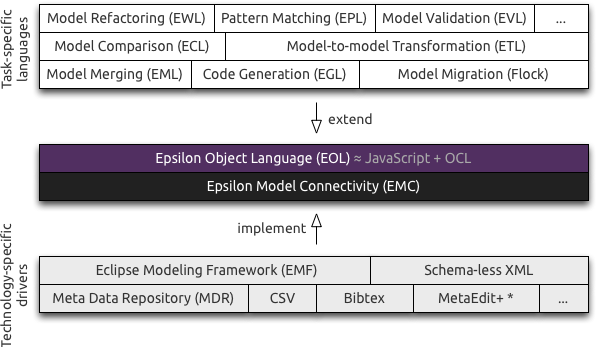
\includegraphics[width=200px]{images/epsilon-architecture}
		\caption{Epsilon Architecture}
	\end{figure}
\end{frame}

\begin{frame}[containsverbatim]
	\frametitle{Example Query and Analysis Code}
\begin{lstlisting}[caption=List authors by number of commits using EpsilonGit, label=lst:exampleCode]
for(author in Author.all.sortBy(a | a.getAllAuthoredCommits().size())) {
	(author.name + " <" + author.emailAddress + ">").println();
}	
	\end{lstlisting}

\begin{lstlisting}[caption=Find Authors who aren't committers, label=lst:exampleCode]
var onlyAuthors = Author.all.excludingAll(Committer.all).sortBy(a | a.getName());
\end{lstlisting}

\begin{lstlisting}[caption=Determine how many merges in repository, label=lst:exampleCode]
Commit.all.reject(c | not c.isMergeCommit()).size().println();
\end{lstlisting}
\end{frame}
\end{document}
